Segunda a \citeonline[p.~5]{e2p}, desde 2000 as fontes renováveis apresentaram um crescimento continuo na matriz energética portuguesa, sobre tudo a geração eólica. Este franco crescimento foi proveniente de uma política europeia e nacional que tem como objetivo a melhoria da segurança de abastecimento, redução da dependência energética e redução dos impactos ambientais do sistema elétrico.  

Como resultado da política energética portuguesa, em 2016  57\% da produção de energia elétrica em Portugal se deu através de fontes renováveis. Face ao ano anterior as fontes renováveis aumentaram 10\% na participação da produção \cite[p.~8]{REN}. O aumento da produção renovável e 2016 deve-se, em parte, da entrada da central hidroelétrica de Frades II, equipada com 780 MW, e do crescimento em 236 MW de potência instalada em parques eólicos portugueses. Seguindo assim uma tendência de crescimento desde 2014, o que pode ser verificada através das estatísticas diária disponibilizadas pela \citeonline{REN-site}.  Em 2016 a geração hidráulica representou 28\% da produção nacional, enquanto a geração eólica representou 22\%, a biomassa representou 5\% e a solar contribuiu com 1\%.

Um fato importante sobre a geração renovável em 2016 é que devido a sua grande participação na produção de energia houve uma redução no preço médio do MWh no mercado ibérico de eletricidade, valor este que esteve situado em 39,4 \euro/MWh \cite[p.~4]{apren}. Comparado ao ano de 2015, quando o custo médio esteve em 50,4 \euro/MWh e a contribuição das renováveis para a matriz energética foi de 48 \%, nota-se uma relação entre o custo \euro/MWh e a  produção renovável. A Figura \ref{fig:CorrelacaoPrecoMercadoProducaoRenovavel} deixa mais explicita esta relação entre o anos de 2015 e 2016.

\begin{figure}[H]
	\centering
	\captionsetup{width=0.85\textwidth, font=footnotesize, textfont=bf}
	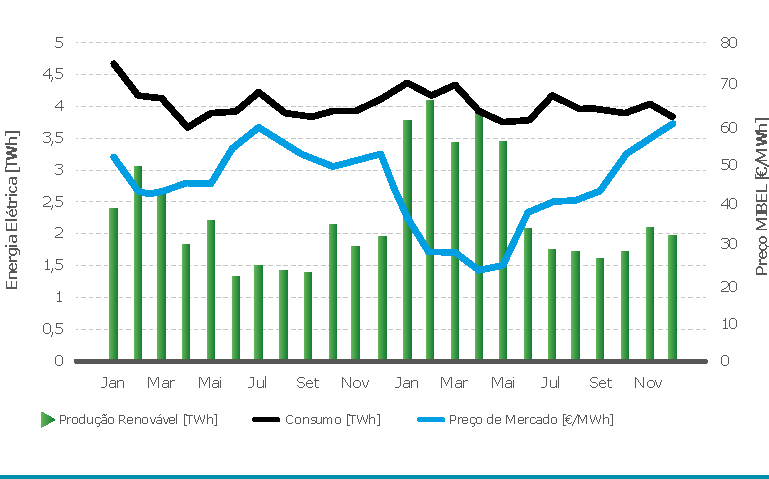
\includegraphics[width=0.8\linewidth]{img/CorrelacaoPrecoMercadoProducaoRenovavel.pdf}
	\caption{Correlação entre o Preço de Mercado e a Produção Renovável (2015-16) }
	\vspace{-3.5mm}
	\caption*{Fonte: \citeonline[p.~10]{apren}}
	\label{fig:CorrelacaoPrecoMercadoProducaoRenovavel}
\end{figure}

Já pelo lado das fontes não renováveis a geração por termoelétricas a carvão e a gás natural ambas representaram, em 2016, 21\% da produção. Face ao ano anterior a produção a carvão sofreu uma queda de 14\%, já a produção a gás natural cresceu 18\% \cite[p.~8]{REN}. Os dados a produção nacional em 2016 estão dispostas Gráfico \ref{fig:ReparticaoDaProducao}, e para fins de comparação está a Tabela \ref{tab:producao20152016}.

\begin{figure}[H]
	\centering
	\captionsetup{width=0.7\textwidth, font=footnotesize, textfont=bf}
	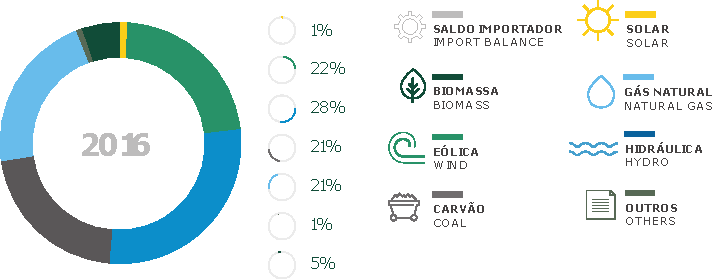
\includegraphics[width=0.7\linewidth]{img/ReparticaoDaProducao2016.pdf}
	\caption{Repartição da Produção}
	\vspace{-3.5mm}
	\caption*{Fonte: \citeonline[p.~8]{REN}}
	\label{fig:ReparticaoDaProducao}
\end{figure}

\begin{table}[H]
	\centering
	\captionsetup{width=0.74\textwidth, font=footnotesize, textfont=bf}
    \begin{tabular}{|l|c|c|c|}
    \rowcolor[HTML]{000000}
    {\color[HTML]{FFFFFF} Geração} & {\color[HTML]{FFFFFF} 2015} & {\color[HTML]{FFFFFF} 2016}   & {\color[HTML]{FFFFFF} Variação(\%) }  \\
    Hídrica                 & 8.453  & 15.413 & 82           \\
    Eólica                  & 11.334 & 12.188 & 8            \\
    Biomassa                & 2.618  & 2.687  & 3            \\
    Solar                   & 760    &  781   & 3            \\
    Carvão                  & 13.677 & 11.698 & -14          \\
    Gás Natural             & 9.807  & 11.571 & 18           \\
    Produção por Bombagem   & 1.160  & 1.217  & 5            \\
    Saldo Importador        & 2.266  & -5.085 & -            \\ \hline
    Produção Não Renovável  & 23.840 & 23.587 & -1           \\ \hline
    Produção Renovável      & 23.165 & 31.069 & 34           \\ \hline
    Produção Total          & 48.165 & 55.873 & 16           \\ \hline
    \end{tabular}
    \caption{Produção Nacional 2015/2016}
    \vspace{-3.5mm}
	\caption*{Fonte: \citeonline[p.~10]{REN}}
    \label{tab:producao20152016}
\end{table}
